%% The first command in your LaTeX source must be the \documentclass command.
%%%% Small single column format, used for CIE, CSUR, DTRAP, JACM, JDIQ, JEA, JERIC, JETC, PACMCGIT, TAAS, TACCESS, TACO, TALG, TALLIP (formerly TALIP), TCPS, TDSCI, TEAC, TECS, TELO, THRI, TIIS, TIOT, TISSEC, TIST, TKDD, TMIS, TOCE, TOCHI, TOCL, TOCS, TOCT, TODAES, TODS, TOIS, TOIT, TOMACS, TOMM (formerly TOMCCAP), TOMPECS, TOMS, TOPC, TOPLAS, TOPS, TOS, TOSEM, TOSN, TQC, TRETS, TSAS, TSC, TSLP, TWEB.
% \documentclass[acmsmall]{acmart}

%%%% Large single column format, used for IMWUT, JOCCH, PACMPL, POMACS, TAP, PACMHCI
% \documentclass[acmlarge,screen]{acmart}

%%%% Large double column format, used for TOG
% \documentclass[acmtog, authorversion]{acmart}

%%%% Generic manuscript mode, required for submission
%%%% and peer review
\documentclass[manuscript, anonymous, review]{acmart}
\usepackage{todonotes}
\usepackage{xcolor}
\usepackage{subfig}
\usepackage{caption}
%% Fonts used in the template cannot be substituted; margin 
%% adjustments are not allowed.
%%
%% \BibTeX command to typeset BibTeX logo in the docs

\AtBeginDocument{%
  \providecommand\BibTeX{{%
    \normalfont B\kern-0.5em{\scshape i\kern-0.25em b}\kern-0.8em\TeX}}}

%% Rights management information.  This information is sent to you
%% when you complete the rights form.  These commands have SAMPLE
%% values in them; it is your responsibility as an author to replace
%% the commands and values with those provided to you when you
%% complete the rights form.
\setcopyright{acmcopyright}
\copyrightyear{2018}
\acmYear{2018}
\acmDOI{XXXXXXX.XXXXXXX}

%% These commands are for a PROCEEDINGS abstract or paper.
\acmConference[Conference acronym 'XX]{Make sure to enter the correct conference title from your rights confirmation emai}{June 03--05,
  2018}{Woodstock, NY}


\acmBooktitle{Woodstock '18: ACM Symposium on Neural Gaze Detection, June 03--05, 2018, Woodstock, NY} 
\acmPrice{15.00}
\acmISBN{978-1-4503-XXXX-X/18/06}


%%
%% Submission ID.
%% Use this when submitting an article to a sponsored event. You'll
%% receive a unique submission ID from the organizers
%% of the event, and this ID should be used as the parameter to this command.
%%\acmSubmissionID{123-A56-BU3}

%%
%% end of the preamble, start of the body of the document source.
\begin{document}

%%
%% The "title" command has an optional parameter,
%% allowing the author to define a "short title" to be used in page headers.
\title{Material Experience Design for Smart Built Environments}

%%
%% The "author" command and its associated commands are used to define
%% the authors and their affiliations.
%% Of note is the shared affiliation of the first two authors, and the
%% "authornote" and "authornotemark" commands
%% used to denote shared contribution to the research.
\author{Shruti Rao}
\email{s.rao@uva.nl}
\orcid{1234-5678-9012}
\affiliation{
  \institution{University of Amsterdam}
  \city{Amsterdam}
  \country{The Netherlands}
}


%%
%% By default, the full list of authors will be used in the page
%% headers. Often, this list is too long, and will overlap
%% other information printed in the page headers. This command allows
%% the author to define a more concise list
%% of authors' names for this purpose.
\renewcommand{\shortauthors}{Rao et al.}

%%
%% The abstract is a short summary of the work to be presented in the
%% article.
\begin{abstract}
%   Abstracts should be about 150 words.

% The digital age is forging a new landscape for architecture where materials and materiality which are closely related to architectural space have undergone a change in their role and how they interact with humans. 

In the digital era of architecture, materials and materiality which are closely related to architectural spaces have changed in their usage and how they interact with humans. The combined use of intelligent technologies with novel materials and design practices in buildings has created unfamiliar human-architecture experiences that remain relatively unexplored. In this position paper, we offer the view of reviewing architecture in the digital age through the lens of the HCI-centric, material experiences framework. We argue that such an approach may be better suited for architecture to understand how materials of today may be used to provide and shape novel human experiences. To that end, we describe our case study within a smart building to understand how occupants perceive, experience and interact with different spaces in the building. Our expected findings may not only aid in understanding subjective human experiences with materials but also identification of specific artefacts that may serve as cues for designing experience-enabling materials in architecture.
\end{abstract}

%%
%% The code below is generated by the tool at http://dl.acm.org/ccs.cfm.
%% Please copy and paste the code instead of the example below.
%%

\begin{CCSXML}
<ccs2012>
   <concept>
       <concept_id>10003120</concept_id>
       <concept_desc>Human-centered computing</concept_desc>
       <concept_significance>500</concept_significance>
       </concept>
   <concept>
       <concept_id>10003120.10003123</concept_id>
       <concept_desc>Human-centered computing~Interaction design</concept_desc>
       <concept_significance>500</concept_significance>
       </concept>
 </ccs2012>
\end{CCSXML}

\ccsdesc[500]{Human-centered computing}
\ccsdesc[500]{Human-centered computing~Interaction design}

%%
%% Keywords. The author(s) should pick words that accurately describe
%% the work being presented. Separate the keywords with commas.
\keywords{architecture, smart buildings, subjective occupant experiences, materials experiences framework, body perception}

%% A "teaser" image appears between the author and affiliation
%% information and the body of the document, and typically spans the
%% page.
% \begin{teaserfigure}
%   \includegraphics[width=\textwidth]{sampleteaser}
%   \caption{Seattle Mariners at Spring Training, 2010.}
%   \Description{Enjoying the baseball game from the third-base
%   seats. Ichiro Suzuki preparing to bat.}
%   \label{fig:teaser}
% \end{teaserfigure}

 
%%
%% This command processes the author and affiliation and title
%% information and builds the first part of the formatted document.
\maketitle

\section{Introduction}
% Architecture + smart buildings
Digital technologies and sustainability sciences are changing the landscape of architecture, and enabling buildings into thoughtful, sustainable and interactive spaces  \cite{kolarevic2004architecture}. Moreover, with digital interactivity becoming a coveted design requirement, ``smart built environments" are a natural outcome in the future of architecture. 

% Materials in Architecture and buildings
\todo{some citations from BxM}
Throughout the discourse of architecture, materials have been considered the language and expression of buildings \cite{schropfer2012material}. However, advancements in technology have dramatically enhanced material capabilities that can now be used to simulate, infer, inform and even create \cite{schropfer2012material, kolarevic2004architecture}. This has resulted in questioning the role of materials in contemporary architectural practices, and how they can be conceived, designed, and produced. 
% Therefore, new material development and changing technological capabilities have questioned the traditional role of materials and materiality as means of expression in architecture.

% Role of humans (body) in architecture and materials
The human body lies at the intersection of architecture and materials that coalesce to interact with the human. The changing nature of materials and therefore the spaces that encompass them may create unfamiliar and novel human-human and human-building interactions that warrant further exploration. These smart buildings especially present an opportunity for human-computer interaction (HCI) research to bridge the gap between intelligent designs, architecture and human needs in such built environments \cite{nembrini2017human}.  

% position
As the relationship between human and architecture enables for a new way of sensory perception of spaces, in this position paper we consider an HCI-based approach on materials and materiality. We posit that architecture in the digital age should be examined through the lens of the material experiences framework. We believe that architecture can benefit from understanding how materials in smart buildings may be used to provide and shape novel human-building and human-human experiences  \cite{giaccardi2015foundations, thomas2006material}. 


% % paper outline
% We next provide relevant background on architecture in the digital age and the material expressions framework. The remainder of this paper then describes our case study as a first step towards understanding the role of materiality of artifacts in architecture, and the contributions our findings can make towards occupant experiences derived from materials in smart buildings.


\section{Background}
% Buildings in the digital age
Architecture in the digital era envisions its role as a communicative tool that can shape the way of perceiving and thinking using an aggregation of materials in a novel fashion \cite{kolarevic2001designing}. In this context, there are several works that try to combine the material with the immaterial (digital) based on the environment. Smart building facades for example are being developed that adapt to the external environment and react in an energy efficient manner \cite{ahmed2015development}. There are also several works that look at providing comfort to users using responsive materials that react to temperature, light, humidity and air quality \cite{fragkia2020exergy, holstov2015hygromorphic, kroner1997intelligent}. 

% Experiences Framework
On the other hand, materials that can shape digital and physical interactions have encouraged human-computer interaction (HCI) research to formalise our understanding of materials and material experiences. The materials experience framework by Giaccardi and Karana (2015) describes three key concepts of \textit{people}, \textit{practises} and \textit{materials}. The authors thereby describe how these three concepts interact to form \textit{relationships}  (encounters,collaborations, and performances) at different \textit{experiential levels} (sensorial, interpretive, affective and performative) \cite{giaccardi2015foundations}. 

% Our perspective
As architectural practises of today show a clear indication of incorporating materials to blend digital experiences with buildings, we wish to examine the relationship between such materials and occupants' experiences in the building following the materials expressions framework. We find it imperative to understand how materials can shape different subjective occupant experiences in architectural spaces.


% Comfort in Architecture
% The concept of comfort is central to occupants within built environments. Comfort is understood as occupants' physiological and affective (emotional) responses to the built environment \cite{alavi2017comfort}. HBI especially examines the relationship between occupant comfort and four physical characteristics of the indoor environment - temperature, air, light, and sound \cite{hawkes2007environmental, bluyssen2009indoor}. 



\section{Towards Material Experiences for Architecture in the Digital Age}

% Why should we design keeping in mind materiality
A significant consequence of smart buildings is that occupants find themselves physically immersed within a digital space, and therefore experience interactions in a novel, multi-sensory manner \cite{nembrini2017human}. We believe that the materials experience framework may be used as a human-centric tool to understand the relationship between materials and occupants at different experiential levels (sensorial, affective, interpretive and performative) within smart buildings \cite{giaccardi2015foundations}. For instance, different tangible and intangible materials in buildings can be utilised to shape the ways in which occupants perceive and experience the building spaces. Moreover, occupant interactions with non-digital elements of the building remains a challenge in HCI and architecture \cite{nembrini2017human}. Carefully designed materials and thereby their experiences can be used to play a more ubiquitous role in fostering occupants' interactions with non-digital elements of the building through digital means
 

\subsection{A Digital Building of the Present}
Our motivation to understand the ``human-building-material" interaction comes from occupying and experiencing one such digital building that houses students, researchers, entrepreneurs, and businesses. The building labelled as an ``intelligent hub" was designed with a very specific architectural vision to be sustainable, circular and flexible, healthy, and inspiring \footnote{https://lab42.uva.nl/}. To that end, different artifacts in the interior and exterior have been designed using a variety of materials and design features. The building facade itself comprises a pattern of open and closed panels that converge towards the top of the building, referencing a binary code. On the inside, wooden laminated beams contrast floors of recycled concrete. The building aims to encourage meeting and communication in the lower floors - a glass atrium is used to indicate the feeling of transparency to occupants who can view all ongoing activities of the building. A combination of colourful plinth is designed to make occupants feel curious and stimulate meeting and collaboration. Quiet and high-concentration in the upper zones are indicated by recycled felt fashioned into panels and inner walls to promote acoustics. A combination of intelligent sensors throughout the building control light, temperature, and air quality to provide for comfort based on available number of occupants, and environmental conditions. 

\begin{figure}[htbp]
\centering
\subfloat[Privacy enabling curtains in a high concentration zone\label{fig:curtain}]{\includegraphics[width=0.2\textwidth]{images/privacy-curtains.jpg}}\hfill
\subfloat[Sheer fabric of the curtains questions the privacy-providing aspect.\label{fig:curtain-sheer}] {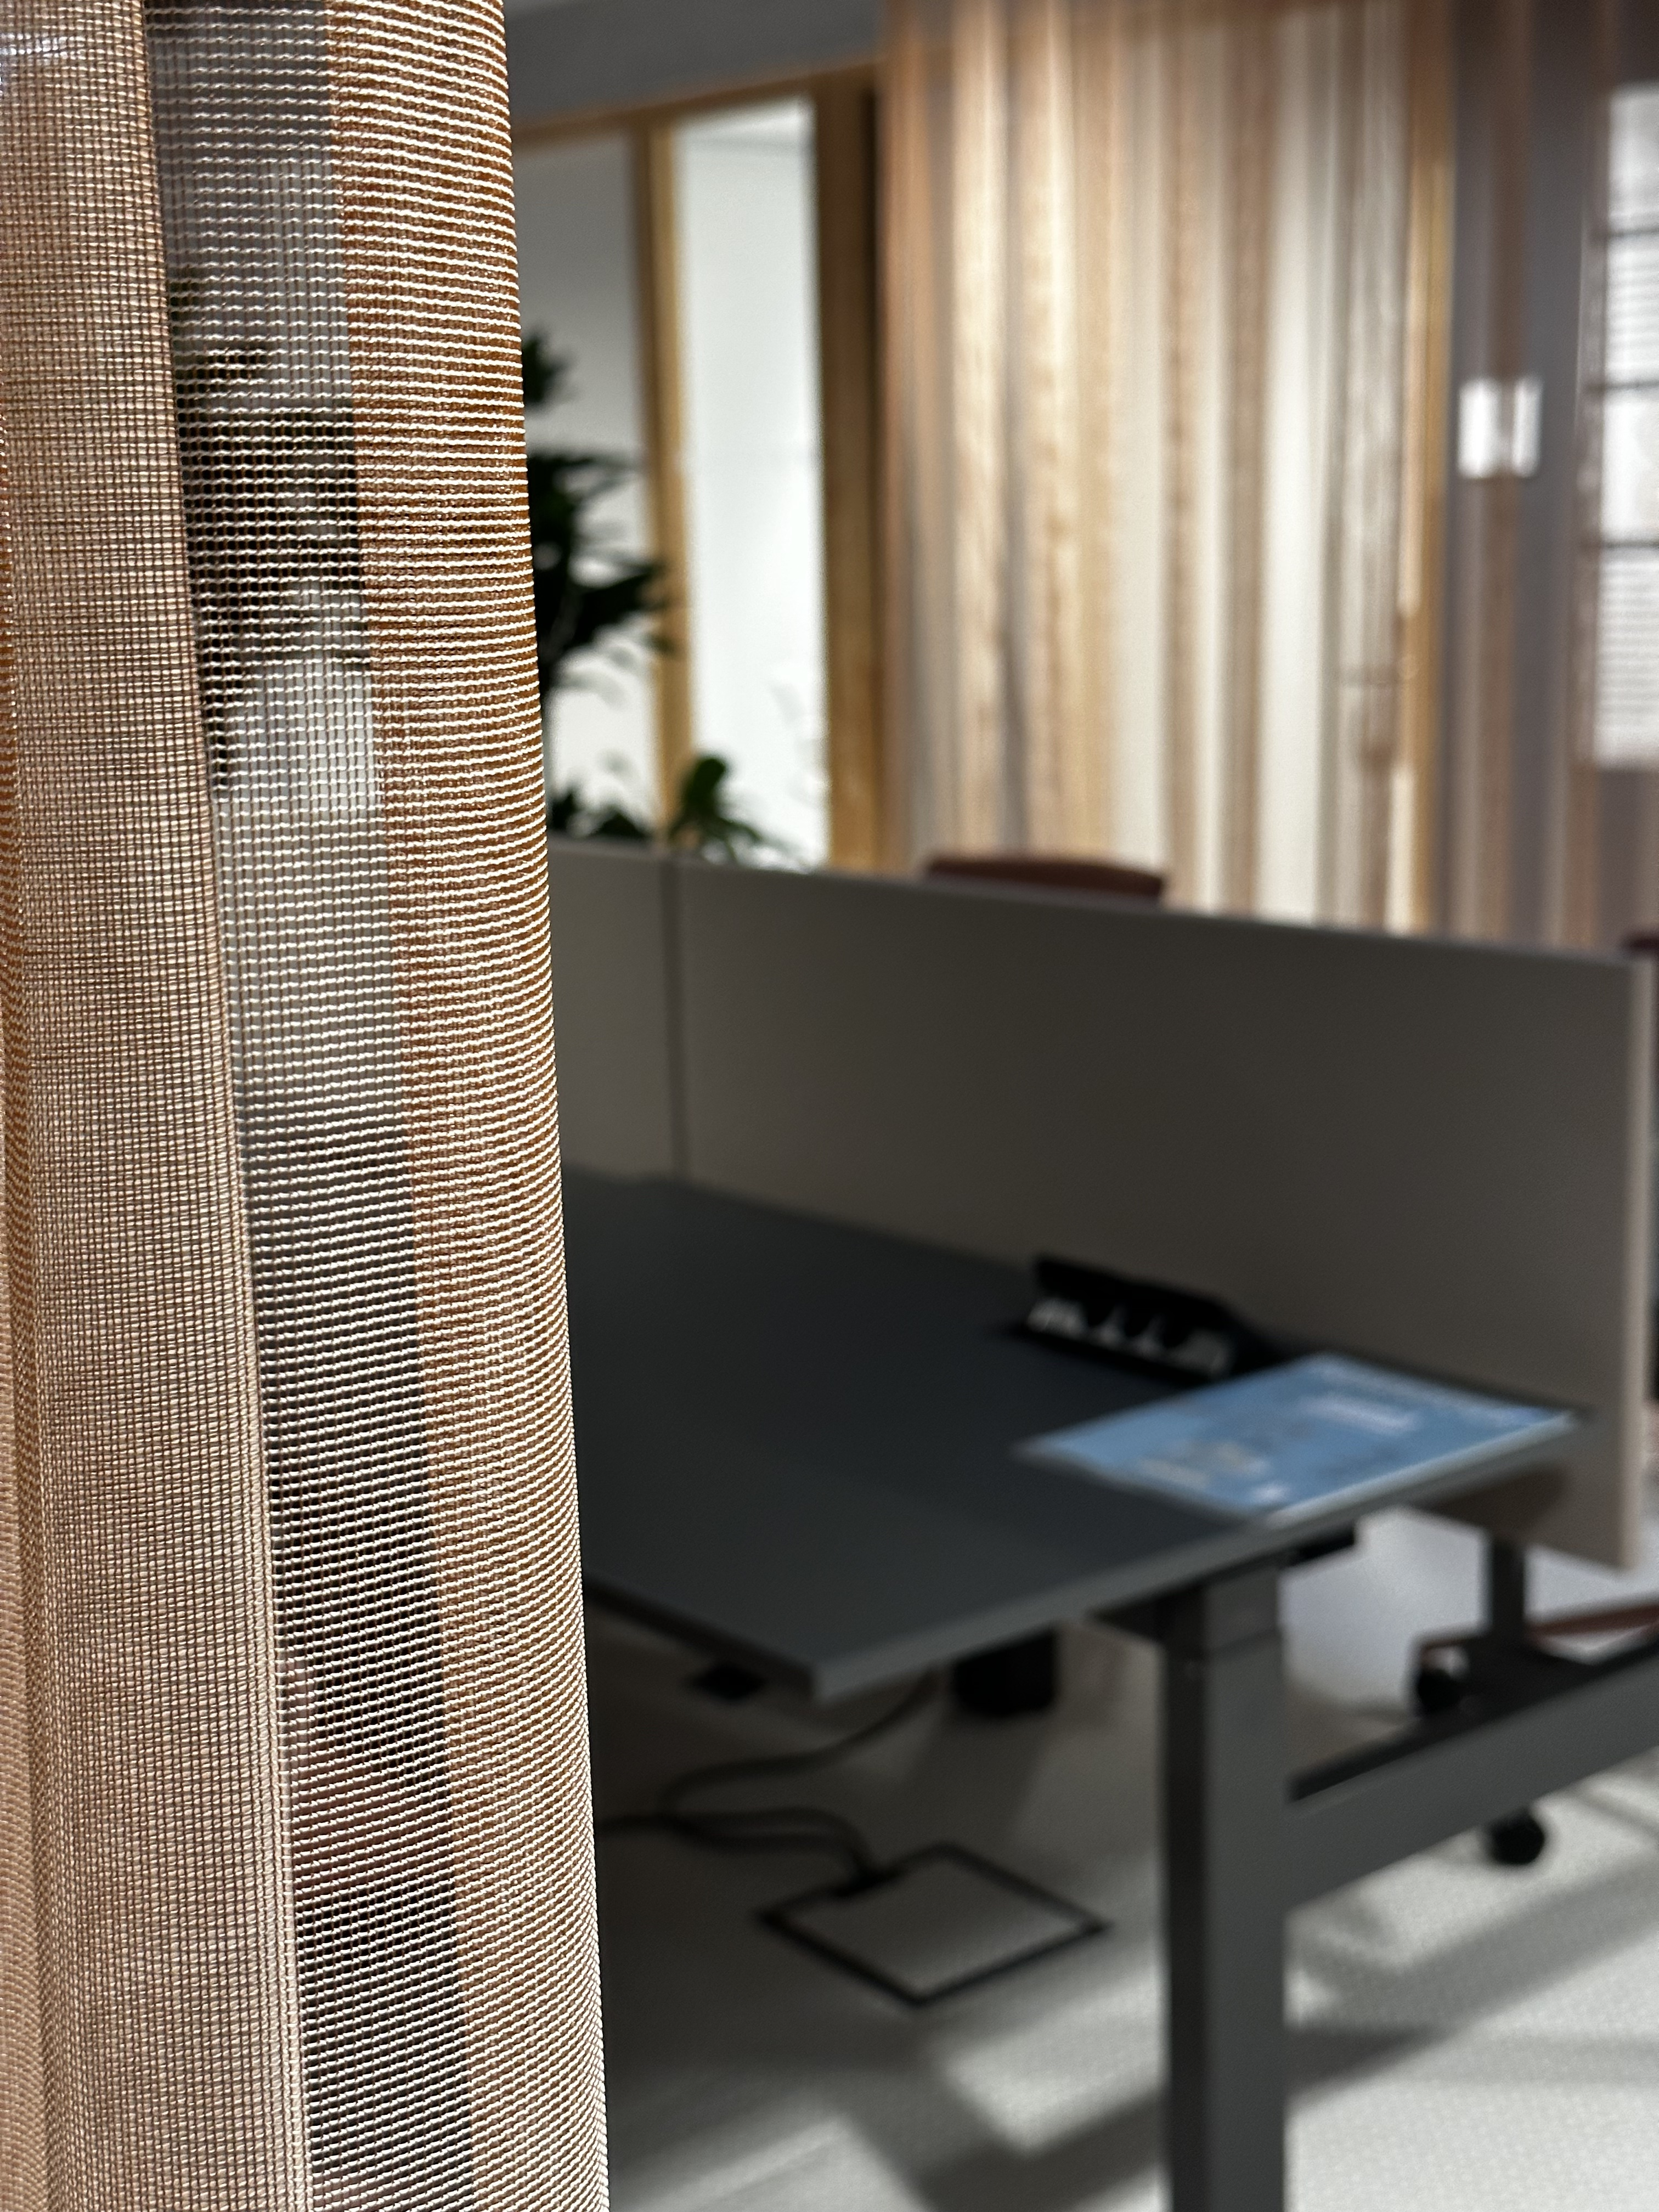
\includegraphics[width=0.2\textwidth]{images/privacy-curtains-fabric.jpg}}\hfill
\subfloat[The building staircase designed to encourage users to take the stairs.\label{fig:staircase}]{\includegraphics[width=0.2\textwidth]{images/stairs.jpg}}\hfill
\subfloat[Wrought iron railings and smooth black surfaces \label{fig:staircase-railing}]{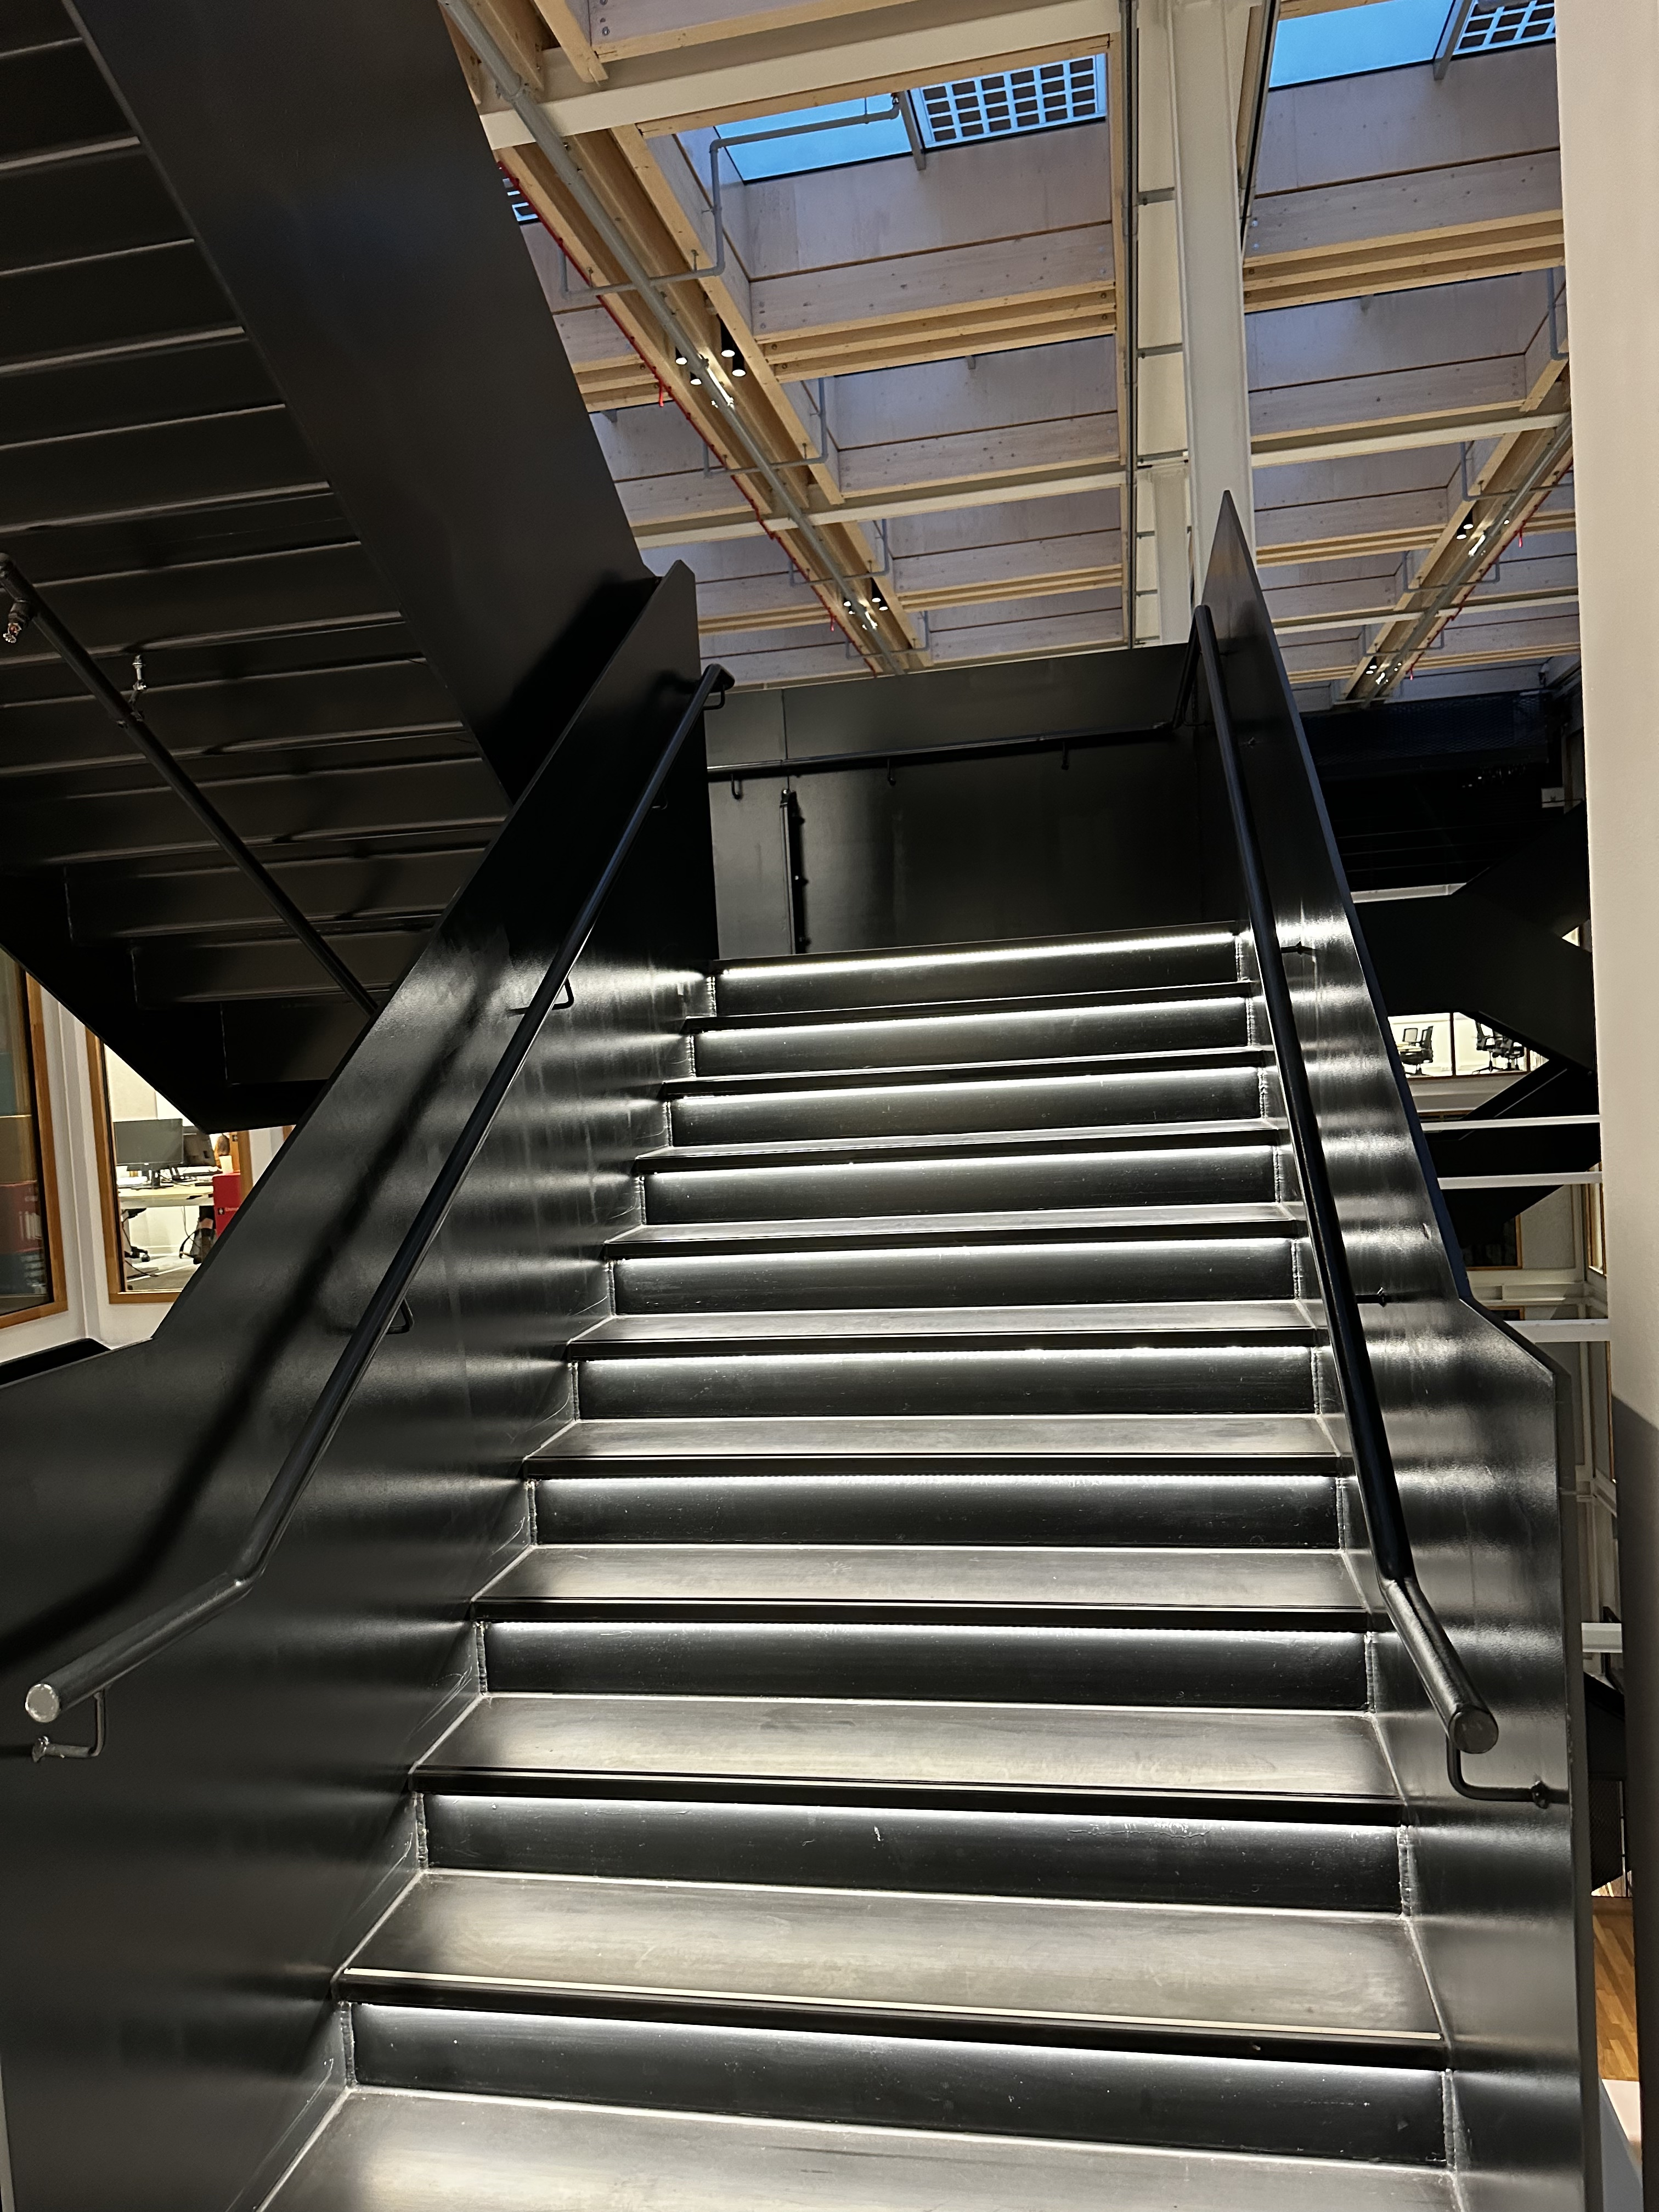
\includegraphics[width=0.2\textwidth]
{images/stairs-closeup.jpg}}
\subfloat[A large screen upon entering the building that serves as a means for communication \label{fig:screen}]{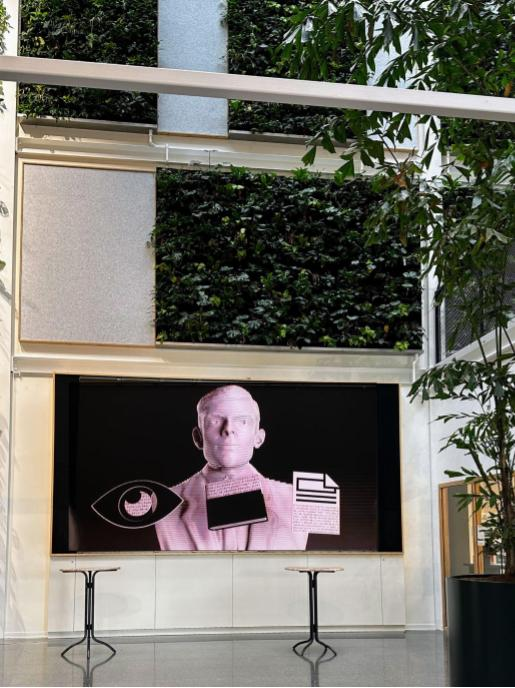
\includegraphics[width=0.2\textwidth]
{images/screen.jpg}}
\caption{Materials in a smart building that raise questions about its nature and the type of experience it provides to the buildings occupants.} \label{fig:lab42-examples}
\end{figure}

Figure \ref{fig:lab42-examples} shows three tangible artifacts in the building designed to provide experiences using a combination of design and materials, but raise questions about the nature of their role in interacting with the building occupants. We speculate on the analysis of material experiences pattern by applying the different levels of the materials experiences framework.

\subsubsection*{The Privacy Curtains}
Figures \ref{fig:curtain} and \ref{fig:curtain-sheer} shows curtains around high-concentration work spaces. The curtains themselves invoke an immediate association with privacy around the workspace (\textit{sensorial level}). However, upon further examination, the sheer material instils a feeling of transparency (\textit{interpretive level}). Therefore, the clash between the concept of privacy and a sheer curtain creates a feeling of confusion and frustration regarding its purpose (\textit{affective level}). However, the physical task of drawing the curtain aids in indicating the need for privacy (\textit{performative level}). So while the curtains itself enable the concept of privacy, the materials used  create an affective discord. We envision an alternative, smart fabric that can intelligently transform from sheer to fully opaque to in-situ cater to privacy needs.

\subsubsection*{An Encouraging Staircase}
The building promotes its staircase in Figures \ref{fig:staircase} and \ref{fig:staircase-railing} as being designed to inspire people to climb stairs rather than use a lift. However, cold and textured wrought iron railings discourages one from using it (\textit{sensorial level}). The black, oversized, and floating structure floating, casts a foreboding  shadow on the onlooker  (\textit{interpretive level}) and the brutalist design evokes a feeling of awe - something to observe, rather than use (\textit{affective level}). We find that the staircase often fails to create a feeling of encouragement and push towards using it.

\subsubsection*{The Digital Interface to the Building}
\todo[]{Try to add images of interface and screen in use}
A large screen in the building foyer accompanied by an interactive interface allows users to explore and learn different things about the building. The interface is an interactive tablet that can be accessed by clicking and moving information around (\textit{sensorial level}). The screen presents itself a digital building attempting to be transparent and communicate with its occupants (\textit{interpretive level}). This placement triggers intrigue in learning more about the building (\textit{affective level}). However, limited information displayed prevents the device from becoming part of an occupant's daily practice (such as checking one's phone every morning) (\textit{performative level}). 

% Our proposed case study
\subsection{Our Proposed Case Study} 
Towards understanding the impact of digital and non-digital materials on occupants in smart buildings, we are undertaking a preliminary case study in the aforementioned building. We aim to identify occupants' novel and subjective experiences that arise from interactions within the smart building. We are particularly interested in understanding experiences of occupant comfort (environmental) and emotions \cite{alavi2017comfort} which is key in built environments.  We wish to thereafter identify specific influential factors (tangible and intangible) that determine the overall sense of comfort and emotions in smart buildings spaces. The case study comprises two phases: (a) emotion and comfort label collection, and (b) building walk. First, we will conduct a short survey to obtain a large number of occupant emotion and comfort information based on different spaces in the building. Next, a building walk will be organised to obtain an in-depth understanding of occupants' perceptions - mental, emotional and physical towards different spaces in the building. During the walk, researchers will engage participants in conversations about each space, and conversations will follow the materials experience framework to understand the relationship between materials, occupants and practises within the different spaces of the building \cite{giaccardi2015foundations}. Questions will also investigate the four different experiential levels (sensory, interpretive, affective and per formative) and will include asking about impressions of the space, usage of space \textit{(How would you use this space? Why do you use this space? What kind of tasks would you perform in this space?)}, emotions in the space \textit{(What emotions do you associate with this space?)}, comfort \textit{(Is this space comfortable? Is there sufficient light, warmth, ventilation?)}, shortcomings and scope for improvement. Participants will also be encouraged to take photos of artifacts that stand out to them. Data collected from both phases will be analysed using thematic analysis, and lexical analysis \cite{braun2006using, xue2020mood}. 


% Expected outcomes that can inform B X M research - Material as a catalyst for human action
\subsection{Expected Contributions}
Through our case study, we aim to (among other goals) identify specific artifacts both tangible and intangible, and the material properties of these artifacts that impact building occupants. Additionally, we expect to gain an understanding of the lived-in bodily comfort and emotional experiences within smart buildings. We believe that our findings may help put forth considerations for designing for occupants needs in smart buildings through the lens of material experiences framework. Our work is a preliminary step towards design and development of materials that can help create experiences that occupants might find lacking in smart buildings (for eg., sense of autonomy and control in an automated building) \cite{moreno2014user}, or enhance certain other experiences (for eg., feeling of groundedness and familiarity in a space used by many) \cite{rehman2022personalisedcomfort}.  For example, smart spaces could be designed with materials that in-situ infer occupants (negative) affective states, and attempt to alter it through means of emapthic responses. 

We ultimately envision a design philosophy for architecture of the digital era that allows material-occupant experiences to shape technology and the ``smartness" of the space. We wish to use our case study to initiate a discussion about creating material-occupant experiences in architecture.


\section{Conclusion}
Digitisation of the architectural landscape in recent years can be attributed to a growing expectation for buildings to adapt to changing socio-environmental and technological needs. Materials that encompass such built spaces and thereby the occupants that inhabit such spaces face a novel relationship. Given the inevitable growth of smart buildings, in this position paper we suggest that materials of a space can play a central role in understanding and shaping occupants experiences towards more human-centric smart buildings. We discuss how materials (both tangible and intangible) of smart buildings can be examined, understood and thereby designed for occupants' subjective needs and experiences following the materials experiences framework. To that end, we highlight a case study that we will undertake to identify understand the impact of one such smart building and it's artifacts (tangible and intangible) on its'  occupants, and therefore needs rethinking and redesign such that they may serve as catalysts for improved human experiences of comfort and wellbeing. 

\bibliographystyle{ACM-Reference-Format}
\bibliography{affective-comfort}

%%
%% If your work has an appendix, this is the place to put it.

\end{document}
\endinput
%%
%% End of file `sample-authordraft.tex'.


% \section{Figures}

% The ``\verb|figure|'' environment should be used for figures. One or
% more images can be placed within a figure. If your figure contains
% third-party material, you must clearly identify it as such, as shown
% in the example below.
% \begin{figure}[h]
%   \centering
%   \includegraphics[width=\linewidth]{sample-franklin}
%   \caption{1907 Franklin Model D roadster. Photograph by Harris \&
%     Ewing, Inc. [Public domain], via Wikimedia
%     Commons. (\url{https://goo.gl/VLCRBB}).}
%   \Description{A woman and a girl in white dresses sit in an open car.}
% \end{figure}

% \subsection{The ``Teaser Figure''}

% A ``teaser figure'' is an image, or set of images in one figure, that
% are placed after all author and affiliation information, and before
% the body of the article, spanning the page. If you wish to have such a
% figure in your article, place the command immediately before the
% \verb|\maketitle| command:
% \begin{verbatim}
%   \begin{teaserfigure}
%     \includegraphics[width=\textwidth]{sampleteaser}
%     \caption{figure caption}
%     \Description{figure description}
%   \end{teaserfigure}
% \end{verbatim}
